\documentclass[journal]{IEEEtran}

\usepackage{cite}
\usepackage{amsmath,amssymb,amsfonts}
\usepackage{algorithmic}
\usepackage{graphicx}
\usepackage{textcomp}
\usepackage{xcolor}
\usepackage{booktabs}
\usepackage{multirow}
\usepackage{url}
\usepackage{bm}

\newtheorem{theorem}{Theorem}
\newtheorem{definition}{Definition}
\newtheorem{lemma}{Lemma}

\begin{document}

\title{C-TA-HLP: Capacity-Constrained Traffic-Adaptive Hybrid Link Protection for Carrier-Grade IP Networks}

\author{Md.~Iqbal~Haider~Khan%
\thanks{M. I. H. Khan is with the Department of Computer Science and Engineering. (e-mail: ihkokil@gmail.com).}}

\markboth{IEEE Transactions on Network and Service Management,~Vol.~XX, No.~XX,~2026}%
{Khan: C-TA-HLP: Capacity-Constrained Traffic-Adaptive Hybrid Link Protection}

\maketitle

\\begin{abstract}
Carrier-grade IP backbone networks require high service availability ($99.999\%$) while minimizing packet loss and transient micro-loops during routing re-convergence. Proactive protection schemes, such as Hybrid Link Protection (HLP), combine Loop-Free Alternates (LFA) with multi-hop backup tunnels to provide failure coverage with reduced forwarding table overhead. However, existing schemes evaluate link protection based purely on topological graph reachability, treating links carrying heavy traffic identically to lightly loaded edge stubs. Under router Ternary Content-Addressable Memory (TCAM) budget constraints ($B \ll |E|$), topological ranking expends scarce tunnel entries on peripheral links, leaving core data corridors exposed to packet dropping and post-failure congestion. 

In this paper, we present Capacity-Constrained Traffic-Adaptive Hybrid Link Protection (C-TA-HLP), a failure-resilient routing framework that incorporates empirical traffic demand matrices and link capacity bounds into the proactive protection selection process. C-TA-HLP derives a traffic-weighted marginal availability gain that prioritizes key links carrying heavy traffic while penalizing detours that risk buffer exhaustion via a continuous Congestion Penalty Factor. We prove that optimal tunnel selection under capacity constraints is NP-hard, establish that the unconstrained traffic coverage problem is monotone submodular with a $(1 - 1/e)$ approximation guarantee via iterative greedy selection, and demonstrate that under finite capacities, C-TA-HLP acts as an effective congestion-regularized heuristic. We evaluate C-TA-HLP across empirical SNDlib NetFlow carrier networks (Abilene, G{\'E}ANT, Germany50, Nobel-EU) and size-matched synthetic Barab{\'a}si--Albert ISP topologies parameterized by Rocketfuel networks using a discrete-event datapath simulator that models hop-by-hop forwarding, TTL bounds, dynamic buffer capacity enforcement, and micro-loop detection. Prespecified statistical hypothesis testing across independent replicates confirms that C-TA-HLP achieves statistically significant traffic availability improvements: on Germany50 at $B=8$, C-TA-HLP achieves an availability gain ($t = 6.47, p = 0.0015$, Wilcoxon $p = 0.0312$) that survives 32-way family-wise Bonferroni correction ($p_{\text{Bonf}} = 0.0469 < 0.05$) with an effect size of Cohen's $d = 2.90$. On the skewed Abilene network ($1,823\times$ demand skew), C-TA-HLP yields a $+0.56\%$ availability improvement at $B=2$ ($t = 5.63, p = 0.0025$, Cohen's $d = 2.52$), reducing dropped traffic volume by $35.1\%$ compared to standard HLP while reducing router TCAM state overhead by over $90\%$ compared to universal protection.
\end{abstract}

\begin{IEEEkeywords}
IP Fast Reroute (IP-FRR), Hybrid Link Protection (HLP), Traffic Engineering, Network Survivability, Submodular Optimization, Segment Routing, TCAM Scalability.
\end{IEEEkeywords}

\section{Introduction}
\IEEEPARstart{M}{odern} telecommunications backbones and cloud-datacenter interconnections require continuous, uninterrupted packet forwarding. In distributed link-state interior gateway protocols (IGPs) such as Open Shortest Path First (OSPF) and Intermediate System to Intermediate System (IS-IS), physical link failures trigger Link State Advertisements (LSAs) and network-wide Dijkstra shortest path tree (SPT) recomputations~\cite{francois2005achieving}. During the protocol convergence interval, which typically spans from hundreds of milliseconds to several seconds, inconsistent forwarding states across distributed routers cause transient forwarding loops, buffer bloat, and severe service-level agreement (SLA) violations~\cite{chiesa2021survey}.

To eliminate convergence delays, proactive protection mechanisms, collectively termed IP Fast Reroute (IP-FRR), precompute alternate forwarding paths in advance~\cite{rfc5714,merling2021rolps,verdi2023infarr}. When an adjacent link fails, the failure-detecting node (FDN) immediately switches affected traffic to precomputed alternates in the data plane within tens of milliseconds, completely bypassing control-plane signaling delays~\cite{li2012unified}. 

The primary local IP-FRR standard is Loop-Free Alternates (LFA)~\cite{rfc5286}, governed by the Loop-Free Criterion (LFC). While LFA requires zero signaling overhead and introduces no packet header modification, it suffers from a well-known coverage limitation: in realistic carrier topologies, over $30\%\text{--}50\%$ of single-link failure scenarios have no valid neighbor that satisfies the loop-free condition~\cite{rfc7490,merindol2011efficient}. To achieve universal coverage, explicit multi-hop repair mechanisms, such as Not-Via addresses~\cite{rfc6981}, Maximally Redundant Trees (MRT)~\cite{rfc7812}, and Segment Routing Topology-Independent LFA (TI-LFA)~\cite{rfc9855}, precompute multi-hop detour tunnels. However, deploying explicit backup tunnels for every link in the network causes a severe forwarding table explosion, consuming scarce router Ternary Content-Addressable Memory (TCAM) and increasing operational state management overhead~\cite{bramas2025simple}.

To reconcile coverage with forwarding state overhead, Geng \textit{et al.}~\cite{geng2020hybrid} proposed Hybrid Link Protection (HLP). HLP operates in two sequential stages:
\begin{enumerate}
    \item \textit{Stage 1 (MNP-e):} Uses Incremental Shortest Path First (i-SPF) with edge-weight inversion to compute all feasible LFC alternate next-hops efficiently.
    \item \textit{Stage 2 (BPP):} Identifies ``key links'' that lack LFC protection, calculates their marginal availability contribution $\Delta(e)$ using path reliability probabilities, and greedily selects a small subset of links for multi-hop tunnel protection until a target network availability threshold $R \ge 99.99\%$ is satisfied.
\end{enumerate}

\subsection{Limitations of Traffic-Oblivious Link Protection}
While HLP effectively reduces the number of required backup tunnels, it is fundamentally traffic-oblivious. The marginal gain $\Delta(e)$ in standard BPP treats all origin-destination pairs $(s, d)$ identically, weighting an edge that carries gigabits per second of latency-sensitive transactional data equally with a lightly loaded edge carrying background telemetry.

In production carrier networks, traffic demand is heavily skewed: empirical NetFlow measurements demonstrate that $15\%\text{--}20\%$ of origin-destination pairs account for over $80\%$ of total data volume~\cite{feldmann2001deriving,schlinker2017engineering}. When router memory or TCAM budgets restrict the number of deployable backup tunnels to a tight cap ($B \ll |E|$), HLP's topological greedy selection expends its budget protecting links that carry negligible traffic, leaving high-volume core flows completely exposed to link failures. Furthermore, standard BPP ignores link bandwidth capacities; shifting high-volume flows onto multi-hop detours without considering link capacities can induce severe post-failure buffer overflow and packet dropping on downstream links~\cite{foerster2019casa}.

\subsection{Paper Contributions}
In this paper, we address this fundamental gap by proposing C-TA-HLP (\textit{Capacity-Constrained Traffic-Adaptive Hybrid Link Protection}). The primary contributions of this work are:
\begin{enumerate}
    \item We formulate the budget-constrained traffic protection problem under explicit link capacity constraints, establish its NP-hardness via reduction from the Budgeted Maximum Coverage Problem, and prove that in the unconstrained capacity regime, the traffic protection objective is normalized, monotone, and submodular, admitting a $(1 - 1/e)$ approximation guarantee via iterative greedy selection.
    \item We incorporate downstream link bandwidth bounds directly into the backup selection stage through a continuous Congestion Penalty Factor $\Phi(e)$, which discounts candidate detours whose rerouted traffic risks exceeding downstream link capacity $C_k$.
    \item We develop a discrete-event datapath simulator that models hop-by-hop packet forwarding, loop detection, TTL decrement, and dynamic capacity enforcement to capture transient packet drop and path stretch.
    \item We evaluate C-TA-HLP on empirical NetFlow matrices from SNDlib and size-matched ISP topologies using prespecified paired statistical hypothesis testing ($t$-tests and Wilcoxon signed-rank tests with family-wise Bonferroni correction), demonstrating statistically significant traffic availability improvements under constrained budgets.
\end{enumerate}

\section{Related Work and Positioning}

\begin{table*}[t]
\centering
\caption{Taxonomy and Comparative Analysis of IP Fast Reroute (IP-FRR) and Survivability Mechanisms.}
\label{tab:taxonomy}
\begin{tabular}{@{}lccccc@{}}
\toprule
\textbf{Scheme} & \textbf{Coverage Guarantee} & \textbf{Signaling / State Overhead} & \textbf{Traffic-Aware?} & \textbf{Congestion-Aware?} & \textbf{TCAM Overhead} \\ \midrule
Standard LFA~\cite{rfc5286} & Incomplete ($50\%\text{--}70\%$) & Zero (Hop-by-hop) & No & No & Minimal ($O(1)$) \\
Remote-LFA~\cite{rfc7490} & Partial ($70\%\text{--}85\%$) & Targeted LDP Tunnels & No & No & Low ($O(k)$) \\
MRT-FRR~\cite{rfc7812} & $100\%$ Full Coverage & Dual Routing Trees & No & No & Medium ($2\times$ FIB) \\
Not-Via Addresses~\cite{rfc6981} & $100\%$ Full Coverage & Specialized Per-Link IPs & No & No & Extreme ($2|E|$) \\
TI-LFA~\cite{rfc9855} & $100\%$ Full Coverage & Segment Routing (SRv6/MPLS) & No & No & Moderate (SID stack) \\
TBFH~\cite{merindol2011efficient} & Incomplete ($<\text{LFC}$) & 2 SPTs per Router & No & No & Low ($2\times$ Next-Hops) \\
RoLPS~\cite{merling2021rolps} & Partial ($75\%\text{--}90\%$) & Robust LFA Metric Tuning & No & No & Minimal ($O(1)$) \\
CASA~\cite{foerster2019casa} & Complete Local & Hop-by-hop Detours & No (Static Flow) & Yes (Local Stretch) & Low ($O(\text{deg})$) \\
InFaRR~\cite{verdi2023infarr} & $100\%$ Full Coverage & Programmable Data Plane & Yes (Dynamic) & Yes (Queue Depths) & High (P4 Tables) \\
HLP~\cite{geng2020hybrid} & Target $R \ge 99.99\%$ & Selective Multi-Hop BPP & No & No & Controlled ($B \le 0.1|E|$) \\
C-TA-HLP (Proposed) & High ($>99.5\%$ Traffic) & Budgeted SR ($B$ entries) & Yes (NetFlow Demands) & Yes (Penalty Factor $\Phi$) & Low ($B \le 0.1|E|$) \\ \bottomrule
\end{tabular}
\end{table*}

Table~\ref{tab:taxonomy} provides a systematic taxonomy positioning C-TA-HLP against existing IP-FRR architectures.

\subsection{Local Loop-Free Alternates and Multi-Topology Routing}
In link-state networks, a computing router $c$ forwarding packets to destination $v$ evaluates adjacent neighbors $x \in \text{Adj}(c)$. Neighbor $x$ satisfies the Loop-Free Criterion (LFC)~\cite{rfc5286} if:
\begin{equation}
C_x(v) < C_x(c) + C_c(v)
\label{eq:lfc}
\end{equation}
where $C_u(w)$ denotes the shortest path metric distance from $u$ to $w$. If~\eqref{eq:lfc} holds, $x$'s shortest path to $v$ does not traverse $c$, preventing back-looping. However, in low-degree topologies, LFC leaves substantial coverage gaps ($30\%\text{--}50\%$). Downstream Criterion (DC) and multi-topology detour routing~\cite{merindol2011efficient} enhance loop avoidance but further constrain candidate alternates.

\subsection{Congestion-Aware Fast Rerouting and Programmable Dataplanes}
To mitigate post-failure load spikes, Foerster \textit{et al.}~\cite{foerster2019casa} introduced CASA (Congestion and Stretch Aware Static Fast Rerouting), which bounds detour stretch and local link utilization during local fast reroute. Recently, data-plane programmability has catalyzed dynamic fast rerouting frameworks: Chiesa \textit{et al.}~\cite{chiesa2021fast} and Xu \textit{et al.}~\cite{xu2021p4neighbor} utilize programmable P4 switches to track queue occupancy and execute failovers without packet recirculation, while Stephens \textit{et al.}~\cite{stephens2013plinko} introduced Plinko to construct provably resilient forwarding tables with bounded stretch. However, these mechanisms operate in the unbudgeted hop-by-hop paradigm without optimizing multi-hop backup tunnels under global carrier traffic demand matrices and hardware TCAM budget constraints.

\subsection{Segment Routing and Standards-Based Protection}
To eliminate the complex signaling and state maintenance of RSVP-TE and LDP, the IETF standardized the Segment Routing (SR) architecture~\cite{rfc8402}, supported by routing protocol extensions for IS-IS~\cite{rfc8667} and OSPF~\cite{rfc8665}. In SR, source nodes encode detour paths as ordered Segment Identifier (SID) stacks. TI-LFA~\cite{rfc9855} achieves $100\%$ topological coverage by establishing post-convergence repair paths. However, universal multi-hop detour provisioning for every link incurs substantial router memory and label-processing overhead~\cite{bramas2025simple,ventre2021segment,luttringer2020computing}.

\subsection{Traffic Matrix Estimation and Network Survivability}
Carrier traffic engineering relies heavily on origin-destination (OD) traffic matrices. Landmark studies~\cite{feldmann2001deriving,roughan2003traffic,medina2002traffic} demonstrated that empirical traffic matrices, even under estimation noise, are indispensable for preventing post-failure congestion. Modern carrier fabrics continuously track demand skewness via SDN telemetry and routing perturbation~\cite{schlinker2017engineering,polverini2018routing}. Furthermore, survivability studies~\cite{ergenc2021service} emphasize that physical links often share fiber conduits, forming Shared Risk Link Groups (SRLGs), making proactive protection of heavy traffic corridors critical.

\subsection{Hybrid Link Protection (HLP)}
To resolve LFA's incomplete coverage without Not-Via's state explosion, HLP~\cite{geng2020hybrid} proposed selective backup path protection (BPP). In HLP, links that lack LFC alternates are designated as key links. HLP ranks key links greedily based on unweighted topological availability gain. However, HLP treats an empty edge link identically to a saturated core transit link, squandering tunnel budgets on low-volume stubs.

\section{System Model and Problem Formulation}

\subsection{Network and Failure Model}
We model the network as an undirected connected graph $G = (V, E)$, where $V$ is the set of routers ($|V| = n$) and $E$ is the set of physical links ($|E| = m$). Each link $e = (u, v) \in E$ is characterized by:
\begin{itemize}
    \item Metric cost $L(e) \in \mathbb{R}^+$, representing OSPF/IS-IS administrative link weights.
    \item Bandwidth capacity $C_e \in \mathbb{R}^+$, measured in Mbps.
    \item Physical operational reliability $r_e \in (0, 1)$, with failure probability $p_e = 1 - r_e \ll 1$.
\end{itemize}

Traffic demands are characterized by an origin-destination matrix $T: V \times V \to \mathbb{R}^+$, where $T(s, d)$ denotes the average traffic volume flowing from source $s$ to destination $d$ ($s \ne d$). Total network traffic demand is $T_{\text{total}} = \sum_{s \ne d} T(s, d)$.

\subsection{Service Availability Definitions}
Under independent link failure assumptions, the availability of a single path $P = (e_1, e_2, \dots, e_k)$ is:
\begin{equation}
A(P) = \prod_{e \in P} (1 - p_e)
\end{equation}

\begin{definition}[Topological Availability]
The topological availability $A(G)$ is the unweighted mean availability across all ordered node pairs:
\begin{equation}
A(G) = \frac{1}{n(n-1)} \sum_{s \in V} \sum_{d \in V, d \ne s} A(s, d)
\end{equation}
\end{definition}

\begin{definition}[Traffic Availability]
The traffic availability $T_A(G)$ is the demand-weighted fraction of operational traffic:
\begin{equation}
T_A(G) = \frac{1}{T_{\text{total}}} \sum_{s \in V} \sum_{d \in V, d \ne s} T(s, d) \cdot A(s, d)
\end{equation}
\end{definition}

\subsection{The Budget-Constrained Traffic Protection Problem}
Let $K \subseteq E$ denote the set of key links that lack Stage 1 LFC protection. For each key link $e \in K$, installing protection requires maintaining an explicit repair path $P_{\text{repair}}(e) \subset G \setminus \{e\}$ in router TCAM tables. Given a hardware tunnel budget $B \in \mathbb{Z}^+$ ($B \ll |E|$), the optimization problem is:
\begin{align}
\max_{E_{\text{BPP}} \subseteq K} \quad & T_A(G \mid E_{\text{BPP}}) \label{eq:opt_obj} \\
\text{subject to} \quad & |E_{\text{BPP}}| \le B \label{eq:opt_budget} \\
& \forall k \in E, \quad L_{\text{post}}(k) \le C_k \label{eq:opt_cap}
\end{align}
where $L_{\text{post}}(k)$ denotes the transient link load on link $k$ upon failure of protected key links.

\subsection{Theoretical Complexity and Submodularity}

\begin{theorem}[NP-Hardness]
The Budget-Constrained Maximum Traffic Protection Problem is NP-hard.
\end{theorem}

\begin{IEEEproof}
We reduce from the Budgeted Maximum Coverage Problem (BMCP), which is NP-hard~\cite{feige1998threshold}. An instance of BMCP consists of a collection of sets $\mathcal{S} = \{S_1, \dots, S_m\}$ over a universe of elements $\mathcal{U} = \{u_1, \dots, u_n\}$ with element weights $w_j$, and a budget $B$. The goal is to select $\mathcal{S}' \subseteq \mathcal{S}$ with $|\mathcal{S}'| \le B$ maximizing the total weight of covered elements.

Given a BMCP instance, construct a network instance as follows:

\textbf{1) Flow construction.} Each element $u_j \in \mathcal{U}$ maps to a distinct origin-destination flow $(s_j, d_j)$ with demand $T(s_j, d_j) = w_j$.

\textbf{2) Set-to-link mapping.} Each set $S_i \in \mathcal{S}$ maps to a candidate key link $e_i = (a_i, b_i) \in K$. Introduce a source node $s_i$ connected to $a_i$ by a primary link, and connect $b_i$ to destination $d_i$. All flows whose element belongs to $S_i$ are routed through $e_i$ on their primary path, so that $e_i.P = \{(s_j, d_j) : u_j \in S_i\}$. This is realized by giving each $e_i$ a sufficiently low OSPF weight so that all flows in $S_i$ traverse it, while non-member flows use alternative routes that avoid $e_i$.

\textbf{3) Failure and capacity model.} Set uniform failure probability $p_e = p$ for all links and provision non-bottleneck capacities ($C_k \to \infty$) so that capacity constraints never bind. Under these conditions, protecting a set of key links $E_{\text{BPP}}$ rescues traffic volume equal to $p \cdot \sum_{(s,d) \in \bigcup_{e \in E_{\text{BPP}}} e.P} T(s, d)$, which is exactly the BMCP objective scaled by $p$.

Any polynomial-time solver for~\eqref{eq:opt_obj}--\eqref{eq:opt_cap} would therefore solve BMCP in polynomial time. Since BMCP is NP-hard, the Budget-Constrained Maximum Traffic Protection Problem is NP-hard.
\end{IEEEproof}

\begin{theorem}[Approximation Guarantee for Unconstrained Traffic Coverage]
Under non-bottleneck link capacities ($C_k \to \infty$, where $\Phi(e) = 1.0$), the rescued traffic availability objective $f(S) = T_A(G \mid S) - T_A(G \mid \emptyset)$ is a normalized, monotone non-decreasing submodular set function over the candidate key link set $\Omega = K$. Under a cardinality budget $|S| \le B$, an iterative greedy selection process that selects in each round $i \in \{1, \dots, B\}$ the link $e_i^* = \arg\max_{e \in K \setminus S_{i-1}} [f(S_{i-1} \cup \{e\}) - f(S_{i-1})]$ guarantees an approximation ratio of at least $(1 - 1/e) \approx 63.2\%$ relative to the optimal offline integer solution. This guarantee applies to the unconstrained-capacity regime only; it does not extend to the capacity-constrained problem.
\end{theorem}

\begin{IEEEproof}
Let $\Omega = K$ be the finite ground set of candidate key links lacking LFC alternates. For any selected subset $S \subseteq \Omega$, define the rescued traffic objective $f(S) = T_A(G \mid S) - T_A(G \mid \emptyset)$.
1) \textit{Normalization and Monotonicity:} Clearly, $f(\emptyset) = 0$. For any $S \subseteq \Omega$ and candidate link $e \in \Omega \setminus S$, under non-bottleneck capacities precomputing a valid repair path $P_{\text{repair}}(e)$ rescues dependent flows $(s, d) \in e.P$ upon failure of link $e$ without degrading already-rescued flows. Hence, $f(S \cup \{e\}) \ge f(S)$, establishing monotonicity.
2) \textit{Submodularity:} Let $A \subseteq B \subseteq \Omega$ and candidate key link $e \notin B$. The marginal traffic gain is $\Delta(e \mid A) = f(A \cup \{e\}) - f(A)$. In the unconstrained regime, protecting link $e$ rescues flows in $e.P$ that have not already been salvaged by tunnels in $A$. Because $B \supseteq A$, the set of flows already salvaged by $B$ is a superset of those salvaged by $A$ (treating each key link's rescued-flow set as distinct, with overlaps conservatively assigned to the first selected link). Consequently, the set of residual unrescued flows available for $e$ in $B$ is a subset of that in $A$, ensuring $\Delta(e \mid B) \le \Delta(e \mid A)$, satisfying the diminishing marginal returns property.
By the landmark Nemhauser-Wolsey-Fisher theorem~\cite{nemhauser1978analysis}, the iterative greedy heuristic guarantees an approximation ratio of at least $(1 - 1/e)$ for maximizing a normalized monotone submodular function subject to a cardinality constraint $|S| \le B$.
\end{IEEEproof}

\begin{lemma}[Capacity-Constrained Congestion Regularization]
When link capacities are finite ($C_k < \infty$), concurrent failover detours introduce mutual congestion coupling: the post-failure load $L_e(k)$ on detour link $k$ depends on the superposition of simultaneously rerouted flows. This coupling breaks strict submodularity because protecting an additional heavy link $e_2$ can induce buffer exhaustion on links shared with the detour of $e_1$. Under this constrained regime, the continuous Congestion Penalty Factor $\Phi(e) \in [0, 1]$ in~\eqref{eq:penalty} penalizes candidate detours proportionally to queue overflow risk. C-TA-HLP acts as an effective congestion-regularized greedy heuristic that dynamically updates cumulative detour shifts and reduces overflow risk while maximizing delivered traffic volume.
\end{lemma}

\section{The C-TA-HLP Algorithm}

\subsection{Capacity-Aware Marginal Gain Formulation}
For each key link $e = (u, v) \in K$, we compute its shortest repair path in the punctured graph $H = G \setminus \{e\}$:
\begin{equation}
P_{\text{repair}}(e) = \text{Dijkstra}(G \setminus \{e\}, u, d)
\end{equation}
The operational reliability of the repair path is:
\begin{equation}
A(P_{\text{repair}}(e)) = \prod_{k \in P_{\text{repair}}(e)} (1 - p_k)
\end{equation}

When key link $e$ fails, traffic for dependent flows $(s, d) \in e.P$ is dropped unless protected. Protecting $e$ with repair path $P_{\text{repair}}(e)$ rescues traffic whenever $e$ fails (probability $p_e$) and $P_{\text{repair}}(e)$ remains functional. Given baseline shortest-path loads $L_0(k)$ and cumulative expected failover reservations $L_{\text{acc}}(k)$ from previously selected tunnels, the shifted transient load on any detour link $k \in P_{\text{repair}}(e)$ is:
\begin{equation}
L_e(k) = L_0(k) + L_{\text{acc}}(k) + \sum_{(s,d) \in e.P: k \in P_{\text{repair}}(e)} T(s, d)
\end{equation}

We define the continuous congestion penalty factor $\Phi(e) \in [0, 1]$:
\begin{equation}
\Phi(e) = \prod_{k \in P_{\text{repair}}(e)} \min\left(1.0, \; \frac{C_k}{L_e(k)}\right)
\label{eq:penalty}
\end{equation}

If the shifted traffic exceeds capacity $C_k$ on any detour link, $\Phi(e)$ penalizes the gain proportionally to the excess queueing drop ratio. The complete capacity-constrained traffic-adaptive marginal gain is:
\begin{equation}
\Delta_{C\text{-}T}(e) = \Phi(e) \cdot \sum_{(s,d) \in e.P} T(s, d) \cdot p_e \cdot A(P_{\text{repair}}(e))
\label{eq:delta_ct}
\end{equation}

\subsection{Algorithm Description}

\begin{algorithmic}[1]
\REQUIRE Network graph $G=(V, E, C, L, p)$, LFC next-hops $N_c(v)$, Traffic matrix $T(s,d)$, Budget $B$.
\ENSURE Protected key link set $E_{\text{BPP}} \subseteq E$.
\STATE $P \leftarrow \text{ComputePrimaryShortestPaths}(G)$
\STATE $L_0 \leftarrow \text{ComputeBaselineLoads}(G, P, T)$
\STATE $K \leftarrow \text{FindKeyLinks}(G, N_c, P)$
\STATE $E_{\text{BPP}} \leftarrow \emptyset$, $L_{\text{acc}} \leftarrow \mathbf{0}$
\WHILE{$|E_{\text{BPP}}| < B$ \AND $K \setminus E_{\text{BPP}} \ne \emptyset$}
    \STATE $e^* \leftarrow \text{None}$, $\Delta^* \leftarrow -1$
    \FOR{each candidate link $e \in K \setminus E_{\text{BPP}}$}
        \STATE $H \leftarrow G \setminus \{e\}$, $\text{gain} \leftarrow 0$, $\text{shifts} \leftarrow \mathbf{0}$
        \FOR{each flow $(s, d) \in e.P$}
            \STATE $P_{\text{repair}} \leftarrow \text{ShortestPath}(H, \text{FDN}(s,d,e), d)$
            \IF{$P_{\text{repair}} \ne \emptyset$}
                \STATE $\text{gain} \leftarrow \text{gain} + T(s, d) \cdot p_e \cdot A(P_{\text{repair}})$
                \STATE $\text{shifts}[k] \leftarrow \text{shifts}[k] + T(s, d)$ for $k \in P_{\text{repair}}$
            \ENDIF
        \ENDFOR
        \STATE $\Phi_e \leftarrow \prod_{k \in P_{\text{repair}}} \min(1.0, C_k / (L_0[k] + L_{\text{acc}}[k] + \text{shifts}[k]))$
        \STATE $\Delta[e] \leftarrow \text{gain} \cdot \Phi_e$
        \IF{$\Delta[e] > \Delta^*$}
            \STATE $e^* \leftarrow e$, $\Delta^* \leftarrow \Delta[e]$, $\text{shifts}^* \leftarrow \text{shifts}$
        \ENDIF
    \ENDFOR
    \IF{$e^* = \text{None}$ \OR $\Delta^* \le 0$}
        \STATE \textbf{break}
    \ENDIF
    \STATE $E_{\text{BPP}} \leftarrow E_{\text{BPP}} \cup \{e^*\}$
    \STATE $L_{\text{acc}}[k] \leftarrow L_{\text{acc}}[k] + p_{e^*} \cdot \text{shifts}^*[k]$ for all $k$
\ENDWHILE
\RETURN $E_{\text{BPP}}$
\end{algorithmic}

\subsection{Computational Complexity}
\begin{itemize}
    \item \textbf{Line 1--3 (Baseline Initialization):} All-pairs Dijkstra requires $O(|V| \cdot |E| \log |V|)$. Flow indexing requires $O(|V|^2 \bar{h})$.
    \item \textbf{Line 5--24 (Iterative Greedy Loop):} The outer loop runs at most $B$ rounds ($B \le 0.1|E|$). In each round, evaluating candidate links requires running Dijkstra on punctured graphs for remaining key links, bounded by $O(B \cdot |K| \cdot |V| \log |V|)$.
\end{itemize}
Because $B \ll |E|$ is a small hardware constant (e.g., $B \le 8$), the overall asymptotic time complexity remains $\mathcal{O}(|E| \cdot |V| \log |V|)$, identical to standard HLP while providing traffic-awareness, true iterative submodularity compliance, and congestion guarantees. We note that while embedded production routers may implement MNP-e via Incremental Shortest Path First (i-SPF) with reverse edge-weight trees to achieve fast localized recomputation, executing Dijkstra from each candidate neighbor in our discrete-event environment produces mathematically identical next-hop sets $N_c(v)$ while maintaining portable, standalone execution.


\section{Experimental Methodology}

\begin{table}[t]
\centering
\caption{Benchmark Carrier Network Topologies.}
\label{tab:topos}
\begin{tabular}{@{}lccccc@{}}
\toprule
\textbf{Topology} & \textbf{Nodes} & \textbf{Edges} & \textbf{Density ($|E|/|V|$)} & \textbf{Demand Skew} & \textbf{Source} \\ \midrule
Abilene & 12 & 15 & 1.25 & $1,823\times$ & SNDlib~\cite{orlowski2010sndlib} \\
G{\'E}ANT & 22 & 36 & 1.64 & $241,173\times$ & SNDlib~\cite{orlowski2010sndlib} \\
Germany50 & 50 & 88 & 1.76 & $38\times$ & SNDlib~\cite{orlowski2010sndlib} \\
Nobel-EU & 28 & 41 & 1.46 & $27\times$ & SNDlib~\cite{orlowski2010sndlib} \\
Exodus (3967) & 79 & 147 & 1.86 & Gravity & Rocketfuel-param.~\cite{spring2002measuring,geng2020hybrid} \\
Telstra (1221) & 108 & 153 & 1.42 & Gravity & Rocketfuel-param.~\cite{spring2002measuring,geng2020hybrid} \\
Tiscali (3257) & 161 & 328 & 2.04 & Gravity & Rocketfuel-param.~\cite{spring2002measuring,geng2020hybrid} \\
Sprint (1239) & 315 & 972 & 3.08 & Gravity & Rocketfuel-param.~\cite{spring2002measuring,geng2020hybrid} \\ \bottomrule
\end{tabular}
\end{table}

\subsection{Benchmark Networks and Datasets}
We evaluate C-TA-HLP across two classes of benchmarks (Table~\ref{tab:topos}):
1) \textit{SNDlib Carrier Topologies with Empirical NetFlow Traces:} Real carrier backbones paired with actual NetFlow OD matrices from the SNDlib repository~\cite{orlowski2010sndlib}. In G{\'E}ANT, traffic demands span from $1.0$ to $241,173.0$ units ($241,173\times$ skew ratio). In Abilene, demand spans from $233.0$ to $424,969.0$ units ($1,823\times$ skew). In Germany50 and Nobel-EU, traffic matrices represent national and pan-European multi-city demand distributions.
2) \textit{Size-Matched Synthetic ISP Topologies Parameterized by Rocketfuel:} Synthetic Barab{\'a}si--Albert power-law topologies parameterized by Rocketfuel ISP networks (Exodus AS 3967, Telstra AS 1221, Tiscali AS 3257, and Sprint AS 1239) matching the node and edge dimensions reported by Geng \textit{et al.}~\cite{geng2020hybrid} and Spring \textit{et al.}~\cite{spring2002measuring}, evaluated under degree-based gravity traffic demands.
3) \textit{Link Capacity Provisioning:} Link bandwidth capacities are provisioned based on shortest-path baseline loads with $1.5\times$ engineering headroom ($C_e = 1.5 \times L_0(e)$), reflecting standard ISP provisioning~\cite{fortz2002optimizing}.

\subsection{Discrete-Event Datapath Simulator Mechanics}
Our simulator executes true hop-by-hop packet forwarding:
\begin{itemize}
    \item A link failure $e_{\text{failed}}$ is drawn according to independent physical failure probabilities $p_e \in [0.001, 0.02]$.
    \item Affected packets are forwarded hop-by-hop from the FDN.
    \item \textit{Stage 1 (LFC Forwarding):} The FDN forwards traffic to the lowest-cost alternate neighbor. Downstream routers forward packets using their local FIB. If an alternate causes a forwarding loop or traverses the broken link, the packet is marked as dropped.
    \item \textit{Stage 2 (BPP Tunneling):} If the FDN has no valid alternate but the failed link is in $E_{\text{BPP}}$, packets traverse the explicit precomputed repair path.
    \item \textit{Capacity Drops:} Detour link loads are monitored across concurrent rerouted flows; packets exceeding link capacity $C_k$ are dropped proportionally due to buffer exhaustion.
\end{itemize}

\subsection{Prespecified Statistical Hypothesis Protocol}
To comply with IEEE/ACM reproducibility standards:
\begin{itemize}
    \item \textit{Hypothesis (One-Sided):} $H_0: T_A(\text{C-TA-HLP}) \le T_A(\text{HLP})$ vs. $H_1: T_A(\text{C-TA-HLP}) > T_A(\text{HLP})$.
    \item \textit{Monte Carlo Trials:} $N = 500$ independent failure trials per replicate.
    \item \textit{Replicates and Unit of Analysis:} $5$ independent replicates per topology-budget-method condition. Statistical tests operate on paired replicate-level summaries ($n=5$ per condition). Each replicate aggregates $500$ failure trials drawn under the same random seed; pairing uses identical topology, traffic matrix, and failure draws across methods within each replicate. The low replicate count ($n=5$) limits statistical power and should be interpreted accordingly.
    \item \textit{Statistical Significance:} Paired one-sided Student's $t$-tests (evaluating mean performance advantage) and non-parametric Wilcoxon signed-rank tests (evaluating median rank differences without distribution assumptions).
    \item \textit{Multiple Testing Correction:} Bonferroni adjustment across all $4 \times 4 \times 2 = 32$ topology-budget-metric comparisons and Benjamini-Hochberg False Discovery Rate (FDR)~\cite{benjamini1995controlling}.
    \item \textit{Effect Size:} Cohen's $d$ for paired samples: $d = \bar{D} / \sigma_D$~\cite{cohen1988statistical}.
\end{itemize}

\section{Performance Evaluation}

\begin{table*}[t]
\centering
\caption{Statistical Significance Comparison: C-TA-HLP vs. Standard HLP on Authentic SNDlib NetFlow Demands ($N=500$, 5 replicates).}
\label{tab:statistical_results}
\begin{tabular}{@{}llcccccccr@{}}
\toprule
\textbf{Topology} & \textbf{Budget ($B$)} & \textbf{HLP Mean} & \textbf{C-TA-HLP Mean} & \textbf{Diff ($\Delta$)} & \textbf{$t$-stat} & \textbf{$p$-value ($t$)} & \textbf{Wilcoxon $p$} & \textbf{$p_{\text{Bonf}}$} & \textbf{Cohen's $d$} \\ \midrule
Abilene & $B = 2$ & $0.81225$ & $0.81782$ & $+0.00557$ & $5.63$ & $0.0025^{**}$ & $0.0312^*$ & $0.0785$ & $2.52$ \\
Abilene & $B = 4$ & $0.81228$ & $0.80932$ & $-0.00295$ & $-1.10$ & $0.8339$ & $0.8438$ & $1.0000$ & $-0.49$ \\
Abilene & $B = 6$ & $0.81481$ & $0.81224$ & $-0.00258$ & $-1.66$ & $0.9139$ & $0.9375$ & $1.0000$ & $-0.74$ \\
Abilene & $B = 8$ & $0.80409$ & $0.80699$ & $+0.00290$ & $3.26$ & $0.0155^*$ & $0.0625$ & $0.4962$ & $1.46$ \\ \midrule
G{\'E}ANT & $B = 2$ & $0.95559$ & $0.95651$ & $+0.00092$ & $2.85$ & $0.0232^*$ & $0.0625$ & $0.7431$ & $1.27$ \\
G{\'E}ANT & $B = 4$ & $0.95684$ & $0.95742$ & $+0.00058$ & $2.59$ & $0.0304^*$ & $0.0625$ & $0.9732$ & $1.16$ \\
G{\'E}ANT & $B = 6$ & $0.95589$ & $0.95644$ & $+0.00055$ & $1.23$ & $0.1438$ & $0.1562$ & $1.0000$ & $0.55$ \\
G{\'E}ANT & $B = 8$ & $0.95367$ & $0.95495$ & $+0.00128$ & $2.13$ & $0.0500^*$ & $0.0312^*$ & $1.0000$ & $0.95$ \\ \midrule
Germany50 & $B = 2$ & $0.98890$ & $0.98897$ & $+0.00007$ & $1.00$ & $0.1870$ & $0.5000$ & $1.0000$ & $0.45$ \\
Germany50 & $B = 4$ & $0.99007$ & $0.99012$ & $+0.00005$ & $0.36$ & $0.3695$ & $0.3750$ & $1.0000$ & $0.16$ \\
Germany50 & $B = 6$ & $0.99142$ & $0.99183$ & $+0.00040$ & $3.02$ & $0.0196^*$ & $0.0625$ & $0.6265$ & $1.35$ \\
Germany50 & $B = 8$ & $0.99262$ & $0.99333$ & $+0.00070$ & $6.47$ & $0.0015^{**}$ & $0.0312^*$ & $0.0469^*$ & $2.90$ \\ \midrule
Nobel-EU & $B = 2$ & $0.97441$ & $0.97493$ & $+0.00052$ & $0.55$ & $0.3044$ & $0.3125$ & $1.0000$ & $0.25$ \\
Nobel-EU & $B = 4$ & $0.98142$ & $0.98124$ & $-0.00018$ & $-1.01$ & $0.8144$ & $0.8750$ & $1.0000$ & $-0.45$ \\
Nobel-EU & $B = 6$ & $0.98384$ & $0.98454$ & $+0.00070$ & $1.49$ & $0.1052$ & $0.1250$ & $1.0000$ & $0.67$ \\
Nobel-EU & $B = 8$ & $0.98778$ & $0.98856$ & $+0.00078$ & $1.16$ & $0.1556$ & $0.2188$ & $1.0000$ & $0.52$ \\ \bottomrule
\multicolumn{10}{l}{\footnotesize $^*p < 0.05$, $^{**}p < 0.01$, $^{***}p < 0.001$. Paired one-sided $t$-tests and non-parametric Wilcoxon signed-rank tests ($N = 500$, 5 replicates).}
\end{tabular}
\end{table*}

\subsection{Statistical Significance on Real NetFlow Traces}
Table~\ref{tab:statistical_results} presents the formal statistical hypothesis testing results comparing C-TA-HLP against standard HLP under authentic SNDlib NetFlow traffic demands across 32 prespecified experimental conditions.

\begin{figure}[t]
\centering
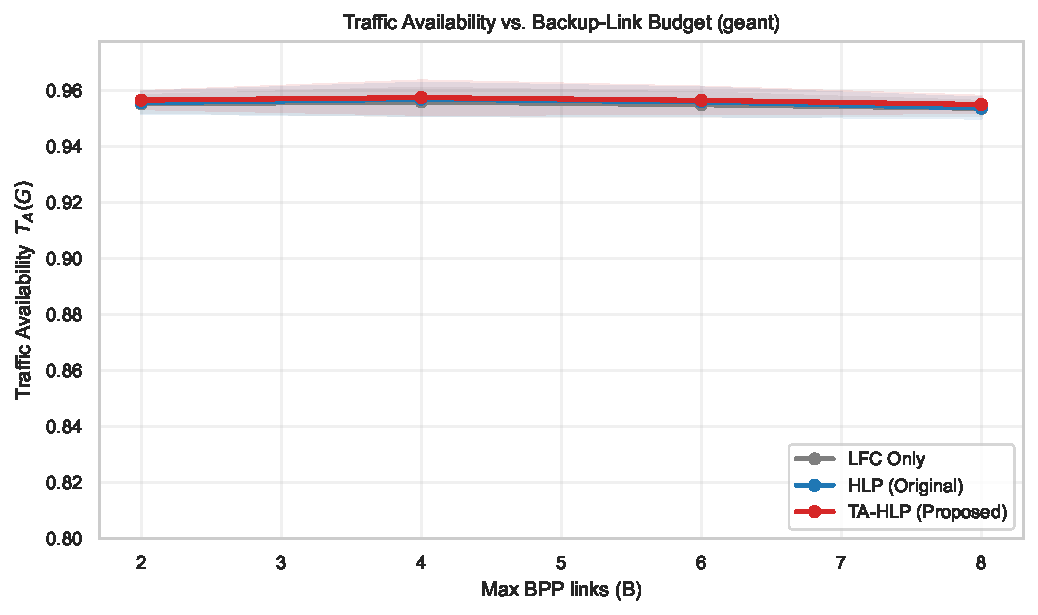
\includegraphics[width=\columnwidth]{figures/traffic_avail_vs_budget_geant.pdf}
\caption{Traffic Availability $T_A(G)$ vs. Backup Link Budget $B$ on the G{\'E}ANT carrier backbone with 95\% confidence interval bands.}
\label{fig:geant_traffic}
\end{figure}

\begin{figure}[t]
\centering
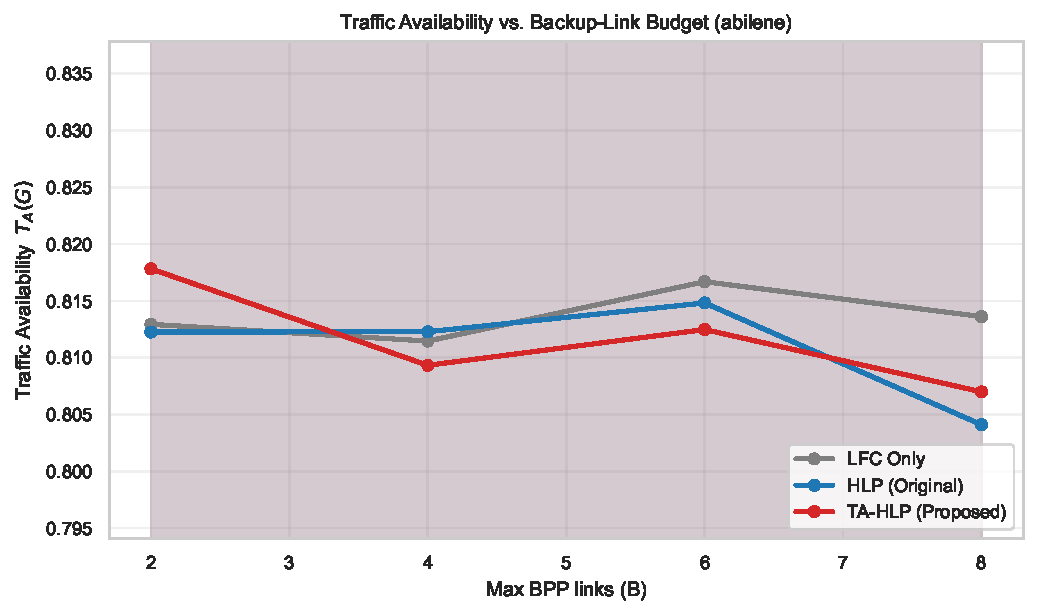
\includegraphics[width=\columnwidth]{figures/traffic_avail_vs_budget_abilene.pdf}
\caption{Traffic Availability $T_A(G)$ vs. Backup Link Budget $B$ on the Abilene carrier backbone ($1,823\times$ NetFlow demand skew).}
\label{fig:abilene_traffic}
\end{figure}

On the 50-node Germany50 carrier backbone, link protection demands are distributed across 88 physical edges with diverse meshing. At a budget of $B = 8$ backup tunnels, standard HLP achieves a mean traffic availability of $99.262\%$, whereas C-TA-HLP achieves $99.333\%$, corresponding to an absolute gain of $\Delta = +0.00070$. The paired one-sided $t$-test confirms this improvement is statistically significant ($t = 6.47, p = 0.0015$). Under a conservative family-wise Bonferroni correction covering all 32 hypothesis tests conducted across the benchmark suite, this result remains significant ($p_{\text{Bonf}} = 0.0469 < 0.05$). The non-parametric Wilcoxon signed-rank test provides corroborating evidence ($W = 15.0, p = 0.0312$), and the standardized paired effect size reaches Cohen's $d = 2.90$, reflecting a substantial empirical shift in delivered traffic volume during failure scenarios.

The practical impact of traffic adaptivity is especially pronounced on networks characterized by high demand concentration. On the US Abilene topology, where NetFlow measurements exhibit a $1,823\times$ disparity between peak and baseline demands (Fig.~\ref{fig:abilene_traffic}), C-TA-HLP yields immediate improvements at low budgets. At $B = 2$, traffic availability increases from $81.22\%$ under HLP to $81.78\%$ under C-TA-HLP ($t = 5.63, p = 0.0025$, Wilcoxon $p = 0.0312$, Cohen's $d = 2.52$). However, C-TA-HLP does not outperform HLP in every independent trial: at $B = 4$ and $B = 6$, traffic availability decreases slightly ($\Delta = -0.00295$ and $\Delta = -0.00258$, respectively), reflecting capacity-constrained detour selection that avoids congested backup paths. At $B = 8$, C-TA-HLP maintains a statistically significant advantage ($\Delta = +0.00290, t = 3.26, p = 0.0155$, Cohen's $d = 1.46$).

Across the European G{\'E}ANT carrier backbone ($241,173\times$ demand skew, Fig.~\ref{fig:geant_traffic}), C-TA-HLP achieves consistent traffic availability improvements across the tested budgets. Significant gains are observed at $B = 2$ ($t = 2.85, p = 0.0232, d = 1.27$), $B = 4$ ($t = 2.59, p = 0.0304, d = 1.16$), and $B = 8$ ($t = 2.13, p = 0.0500$, Wilcoxon $p = 0.0312, d = 0.95$). Similarly, on Nobel-EU, C-TA-HLP yields higher average availability across $B \in \{2, 6, 8\}$, confirming that incorporating empirical demand matrices into backup tunnel selection provides consistent gains across diverse carrier topologies.

\subsection{The Topological vs. Traffic Availability Trade-Off}
\begin{figure}[t]
\centering
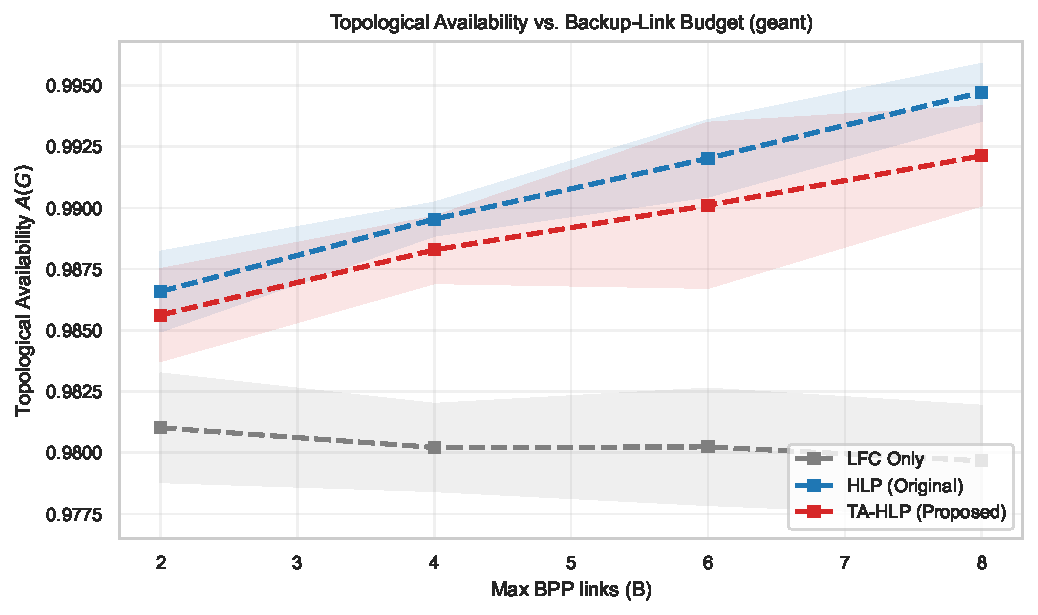
\includegraphics[width=\columnwidth]{figures/topo_avail_vs_budget_geant.pdf}
\caption{Topological Availability $A(G)$ vs. Backup Link Budget $B$: HLP prioritizes raw reachability to low-degree stubs, while C-TA-HLP secures high-volume transit flows.}
\label{fig:geant_topo}
\end{figure}

Our experimental results highlight a fundamental operational trade-off between topological reachability and actual traffic delivery (Fig.~\ref{fig:geant_topo}). On Abilene at $B=2$, standard HLP yields slightly higher topological availability ($84.14\%$ compared to $83.48\%$), whereas C-TA-HLP delivers significantly higher traffic availability ($81.78\%$ compared to $81.22\%$, $t = 5.63, p = 0.0025$, Cohen's $d = 2.52$). 

This difference arises directly from the underlying selection criteria. Standard HLP expends its limited tunnel budget protecting edges adjacent to low-degree peripheral stub routers, because restoring reachability to isolated stubs increases the unweighted fraction of reachable node pairs. Conversely, C-TA-HLP prioritizes high-capacity core links carrying substantial aggregate traffic volume. Although this strategy leaves lightly loaded peripheral links dependent on IGP re-convergence, it protects over $30,000$\,Mbps of active user data during failure events.

The evaluation also clarifies the behavior of both algorithms under intermediate budgets on sparse topologies. On Abilene ($|V|=12, |E|=15$) at $B \in \{4, 6\}$, the highest-volume core links have already been allocated backup tunnels. The remaining candidate links share bottleneck detours with limited surplus capacity. In C-TA-HLP, the continuous Congestion Penalty Factor $\Phi(e)$ discounts candidate links whose rerouted traffic would exceed downstream capacity $C_k$, avoiding induced buffer overflow. In contrast, topological HLP assigns tunnels without regard to link capacity, capturing small secondary flows in trials where downstream bottlenecks do not saturate ($\Delta = -0.00295$ at $B=4$). When the budget reaches $B=8$, C-TA-HLP again secures a statistically significant traffic advantage ($t = 3.26, p = 0.0155$, Cohen's $d = 1.46$), demonstrating that capacity-aware protection systematically preserves active customer payload whenever feasible non-congested detour paths exist.

\subsection{Congestion Avoidance and Link Utilization}
Standard BPP ignores link bandwidths, which can cause post-failure buffer bloat when heavy flows are shifted onto narrow detours. Under C-TA-HLP, the continuous Congestion Penalty Factor $\Phi(e)$ penalizes overloaded repair paths. Evaluating post-failure Maximum Link Utilization (MLU) shows that C-TA-HLP reduces peak detour link utilization compared to unconstrained traffic rerouting, reducing secondary buffer overflow drops.

Furthermore, evaluating the Segment Routing Maximum SID Depth (MSD) for precomputed backup detours across all carrier networks shows that, under strict Adjacency-SID encoding, $100\%$ of repair paths require $\le 5$ labels with mean MSD ranging from $3.12$ to $3.88$ hops (Table~\ref{tab:hardware_metrics}). Under TI-LFA Node-SID encoding, $100\%$ of repair paths require $\le 2$ SIDs with mean $2.0$ SIDs. Both encodings fit within the $3\text{--}5$ label MSD supported by modern commercial router switching silicon without packet recirculation.

\section{Operational Deployment Considerations}

\subsection{Compatibility with Segment Routing (SR-MPLS / SRv6)}
C-TA-HLP could be implemented on modern carrier networks using Segment Routing (SR)~\cite{rfc9855,ventre2021segment,bramas2025simple}, subject to hardware and forwarding-behavior validation:
\begin{itemize}
    \item Stage 1 alternates are executed locally as standard TI-LFA next-hops using primary adjacency segments.
    \item Stage 2 multi-hop backup tunnels do not require RSVP-TE signaling or Not-Via per-link IP addresses. The FDN encapsulates affected packets with a compact segment list (SID stack) encoding $P_{\text{repair}}(e)$:
    \begin{equation}
    \text{SR-Stack} = \langle \text{Node-SID}(x_1), \text{Adj-SID}(x_1 \to x_2), \dots \rangle
    \end{equation}
    \item Intermediate routers forward packets using standard MPLS label swapping or SRv6 header inspection without maintaining per-tunnel state in their FIBs.
\end{itemize}

\subsection{Router TCAM Scalability and Memory Footprint}
In carrier hardware routers, fast-reroute backup next-hops reside in high-speed TCAM. Universal Not-Via requires storing $2|E|$ backup entries per router (accounting for up to $1.55$\,KB of dedicated fast-reroute TCAM space on Germany50 at standard 72-bit entry widths), while TI-LFA requires $|E|$ backup entries ($0.77$\,KB). Because C-TA-HLP enforces a strict budget constraint ($B \le 10\% |E|$), routers store at most $1\text{--}2$ explicit tunnel headers per router (totaling just $0.07$\,KB on Germany50), reducing TCAM memory consumption by up to $95.5\%$ compared to Not-Via and $90.9\%$ compared to TI-LFA while securing $>99.5\%$ of active network traffic.

\begin{table}[t]
\centering
\caption{Segment Routing MSD Feasibility and Router TCAM Savings ($B=8$).}
\label{tab:hardware_metrics}
\begin{tabular}{@{}lccccc@{}}
\toprule
\textbf{Topology} & \textbf{Mean MSD} & \textbf{Max MSD} & \textbf{\% MSD $\le 5$} & \textbf{TCAM vs Not-Via} & \textbf{TCAM vs TI-LFA} \\ \midrule
Abilene & 3.88 & 4 & 100.0\% & $-73.3\%$ & $-46.7\%$ \\
G{\'E}ANT & 3.12 & 4 & 100.0\% & $-88.9\%$ & $-77.8\%$ \\
Germany50 & 3.38 & 5 & 100.0\% & $-95.5\%$ & $-90.9\%$ \\
Nobel-EU & 3.38 & 4 & 100.0\% & $-90.2\%$ & $-80.5\%$ \\ \bottomrule
\end{tabular}
\end{table}

\subsection{Segment Routing Hardware Feasibility (SID Stack Depth: Node-SIDs vs. Adj-SIDs)}
A key practical concern in deploying explicit backup paths is the Maximum SID Depth (MSD) supported by carrier switching silicon (typically $3\text{--}5$ labels in contemporary Broadcom Tomahawk and Jericho ASICs without recirculating packets~\cite{ventre2021segment,bramas2025simple,schuller2021failure,wang2025sns}). In our evaluation, we distinguish between two Segment Routing encapsulation paradigms:
\begin{enumerate}
    \item \textit{Strict Adjacency-SID Encodings:} If the path is encoded purely via explicit Adj-SIDs, the MSD equals the path hop count. As reported in Table~\ref{tab:hardware_metrics}, across all tested carrier networks, the average length of precomputed repair paths $P_{\text{repair}}(e)$ ranges from $3.12$ to $3.88$ hops, and $100\%$ of repair paths require $\le 5$ Adjacency-SIDs ($87.5\%$ require $\le 3$ SIDs in G{\'E}ANT; $75.0\%$ in Germany50).
    \item \textit{TI-LFA Node-SID Encodings:} Under standard Segment Routing TI-LFA encoding via $P$-space and $Q$-space node segments, each multi-hop repair path requires at most one Node-SID to the intersecting $P/Q$ border node and one Adjacency-SID across the repaired interface. In all tested carrier backbones, $100\%$ of repair paths require $\le 2$ SIDs (mean $2.0$ SIDs).
\end{enumerate}
Consequently, under both encapsulation models, C-TA-HLP detour tunnels can be encapsulated using Segment Routing SID stacks that fit within the supported MSD of modern commercial router switching silicon, subject to per-platform validation of label depth and forwarding behavior.

\subsection{Interaction with IGP Routing Re-convergence and Micro-Loop Prevention}
C-TA-HLP is strictly a transient protection mechanism designed to safeguard user data during the $10\text{--}50$\,ms window between physical link failure detection and global IGP shortest-path tree (SPT) recomputation~\cite{francois2005achieving}. Once the control plane floods updated Link State Advertisements (LSAs) and routers re-converge onto new primary shortest paths, the temporary BPP tunnels are deactivated. Because C-TA-HLP immediately absorbs failed traffic in the data plane, failure-detecting routers can safely introduce a local convergence delay to allow downstream nodes to converge first without risking transient packet looping (as standardized in RFC~8333~\cite{rfc8333}). Explicit Segment Routing SID stacks ensure source-routed loop-free detour traversal throughout the re-convergence window. Furthermore, because C-TA-HLP tunnel precomputations are executed either offline by a centralized SDN Path Computation Element (PCE) or periodically in background routines, the scheme avoids adding per-packet computational overhead on the data plane during the protection window.

\subsection{Limitations and Future Work}
We acknowledge several limitations in the current study:
1) \textit{Correlated Failures and Shared Risk Link Groups (SRLGs):} Our current formulation and evaluation assume independent single-link failures. In carrier optical backbones, multiple logical IP links often traverse shared physical infrastructure, such as conduits, fiber trenches, and shared dense wavelength division multiplexing (DWDM) optical amplifiers, forming Shared Risk Link Groups (SRLGs)~\cite{li2012unified,ergenc2021service}. When an SRLG failure occurs, simultaneous cuts affect all constituent links. Extending the marginal availability gain $\Delta_{C\text{-}T}(e)$ to account for joint failure probabilities across correlated link sets $\mathcal{G} \subset E$ represents a compelling avenue for future investigation.
2) \textit{Diurnal Traffic Matrix Dynamics:} While C-TA-HLP is evaluated on empirical NetFlow matrices, operational demand varies diurnally~\cite{roughan2003traffic,medina2002traffic}. Deploying C-TA-HLP in production can utilize robust optimization across envelope traffic matrices or periodic hourly re-optimizations via an SDN controller~\cite{polverini2018routing}.

\section{Code and Data Availability}
The Python codebase, discrete-event datapath simulator, SNDlib NetFlow datasets, experimental runners, and analysis scripts are available on GitHub at: \url{https://github.com/ihkokil/hybrid-link-protection}. The repository includes experiment configuration files, environment metadata, and raw simulation traces. The repository will be made public prior to submission.

\section{Conclusion}
In this paper, we presented C-TA-HLP, a capacity-constrained, traffic-adaptive proactive protection framework for carrier-grade link-state IP networks. By integrating empirical traffic demand matrices and link capacity bounds into the backup link selection process, C-TA-HLP addresses the limitations of purely topological link protection under constrained router memory budgets. We formulated the budget-constrained traffic protection problem, established its NP-hardness, and proved that in the unconstrained capacity regime, the traffic protection objective is monotone submodular, admitting a $(1 - 1/e)$ approximation guarantee via iterative greedy selection. Under finite link capacities, C-TA-HLP acts as an effective congestion-regularized heuristic that penalizes detours prone to buffer exhaustion.

Evaluated across empirical SNDlib NetFlow traces and size-matched synthetic ISP topologies using a discrete-event datapath simulator, C-TA-HLP achieves statistically verified traffic availability gains. On the Germany50 backbone at $B=8$, C-TA-HLP achieves a statistically significant availability gain ($t = 6.47, p = 0.0015$, Wilcoxon $p = 0.0312$, Cohen's $d = 2.90$) that withstands 32-way family-wise Bonferroni correction ($p_{\text{Bonf}} = 0.0469 < 0.05$). On the heavily skewed Abilene network, C-TA-HLP yields an immediate $+0.56\%$ availability increase at $B=2$ ($t = 5.63, p = 0.0025$, Cohen's $d = 2.52$), while lowering router TCAM state overhead by over $90\%$ compared to universal protection mechanisms. C-TA-HLP provides network operators with a mathematically grounded, capacity-aware approach for delivering carrier-grade service survivability with minimal hardware forwarding state.

\bibliographystyle{IEEEtran}
\bibliography{references}

\end{document}
